\documentclass[../main.tex]{subfiles}
\begin{document}

This review explores and synthesizes existing approaches for the evaluation of causal inference estimators. I aim to achieve three primary goals. First, to justify the importance of finite sample evaluation based on Monte Carlo methods by exploring the landscape of alternatives. Second, to establish principles for the validity of finite sample evaluation. Finally, third, to analyze the validity of existing approaches in terms of these principles in order to motivate a better approach. This literature review is comprised of four sections that work toward these goals. First, I briefly establish definitions for statistical inference and estimators which perform this inference. Second, I explore the landscape of different approaches to evaluating the performance of estimators - comparing theoretical, asymptotic evaluation and Monte Carlo-based finite-sample evaluation. Third, I establish the general principles for the validity of finite sample evaluation. Finally, I apply these principles to analyze existing approaches to evaluating causal inference estimators. The first three sections present this author’s framing of the literature with light reference to the underlying works. The final section is a close review of the existing methods of Monte Carlo based evaluation.\par

\section{Statistical Inference and Estimators}

\vspace{\baselineskip}
All statistical inference can be characterized in the following simple terms, due to Pearl (2009, $\#$ ref): There is some true data generating process (DGP) characterized by a set of (random) variables, functions (possibly probability distributions) that relate these variables, and parameters that determine the exact form of the functions. The DGP gives rise to a joint distribution over the variables which make up the DGP. Any sample of observed data can then be thought of as a sample from this joint distribution. The goal of inference is to estimate the functional relationships and parameters of the original data-generating process using sample data from the joint probability distribution.\par


\vspace{\baselineskip}
As summarized in Calder (1953 $\#$ ref), estimators operationalize inference by providing a mathematical mapping between a sample of data from the true joint distribution and an estimate of a target parameter - an \textit{estimand} - that is (or is concretely related to) a parameter from true DGP. Given that a sample is inherently stochastic, estimators give rise to a \textit{sampling distribution }over the estimand rather than a single value. The quality of an estimator is defined by some quality metric that depends on this sampling distribution. Concretely defining the abstract notion of the ‘quality’ of an estimator is a non-trivial task, discussed below.\par

\section{Evaluating the Performance of Statistical Estimators}

\vspace{\baselineskip}
Ultimately, the goal of evaluation is to determine the quality of an estimator. There is no single measure for quality. The metric used is sensitive to the eventual application of the estimator and the real-world, normative value associated with various kinds of error. Bishop (2006, Chapter 1 $\#$ ref) outlines most of the commonly encountered quality metrics and in which circumstances they tend to be most useful. The common thread which unifies these metrics is that they depend on the estimator's sampling distribution over the estimand. All metrics are, at some level of abstraction, calculated in reference to this sampling distribution (Calder, 1953 $\#$ ref). So, the estimator itself, the sample size available, and the underlying joint data distribution affect the value quality metrics by affecting the sampling distribution.\par


\vspace{\baselineskip}
Given the central role of the sampling distribution, one can think about evaluation approaches in terms of how they derive the sampling distribution for a given estimator. In this framing, there are two approaches that I will refer to as \textit{theoretical} and \textit{experimental.} Theoretical methods derive an analytical expression for the sampling distribution based on the estimator, sample size, and underlying data distribution. Experimental approaches \textit{estimate }the sampling distribution by repeatedly applying the estimator to samples from an underlying data distribution with a known value for the estimand. Repeat sampling results in convergence to the expected value of any metric defined over the sampling distribution (Paxton, 2001 $\#$ ref). This provides \textit{experimental} insight into the performance of the estimator in the sense that data is collected to estimate the quality of the metric under researcher-controlled settings of the sample size and underlying distribution. In general, the process of using samples from a distribution to estimate the value of parameters over that distribution is referred to as Monte Carlo estimation (Hastings, 1970 $\#$ ref). This is why sampling-based evaluation is referred to as Monte Carlo Evaluation in the literature.\par


\vspace{\baselineskip}
These two approaches - theoretical and experimental - are not mutually exclusive and, for the evaluation of an arbitrary estimator, can both provide useful information. However, honing in on our specific context, Paxton et al (2001 $\#$ ref) provide a compelling analysis of the specific usefulness of Monte Carlo evaluation in evaluating econometric estimators. They raise three concerns with the usefulness of theoretical evaluation which are outlined below along with corresponding points made by authors who reach the same conclusions with regard to evaluating causal inference estimators specifically.\par


\vspace{\baselineskip}
\begin{enumerate}
	\item In many cases, the theoretical sampling distribution for an estimator is not known. As pointed out in Knaus et al (2018 $\#$ ref), more complex estimators tend to make for much more challenging theoretical analysis. This fact, combined with the trend toward semi/nonparametric causal estimators outlined in the introduction, means that theoretical sampling distributions are missing for many causal inference estimators which have proven promising in practice.\par


\vspace{\baselineskip}
	\item Theoretical evaluation tends to rely heavily on simplifying assumptions - the most common of which is the assumption of the normality of the underlying data distribution. These assumptions limit the applicability of the theoretical sampling distribution: it is unlikely that real-world data distributions meet these assumptions and thus the theoretical metrics may not hold on real data. Even if the assumptions behind the theoretical analysis of different methods are available, Knaus et al (2018 $\#$ ref) point out that the assumptions behind the analysis for different estimators may not overlap such that comparing theoretically derived metric values is impossible.\par


\vspace{\baselineskip}
	\item Theoretical analysis tends to hold in the asymptotic limit of large sample sizes. The implications of theoretical results for finite samples is not necessarily well defined. This is echoed in Huber et al (2013 $\#$ ref).
\end{enumerate}\par


\vspace{\baselineskip}
Taken together, these three weaknesses mean that Monte Carlo analysis - which can be performed using arbitrary sample sizes and on any underlying data distribution - plays a crucial role in the evaluation of causal inference estimators. The rest of this review focuses exclusively on these methods of evaluation, exploring the principles which define a good Monte Carlo evaluation and how existing variants measure up against these principles.\par

\section{Monte Carlo Evaluation of Causal Inference Estimators}
\subsection{General Principles}

\vspace{\baselineskip}
This section proposes a synthesized set of principles for what makes a \textit{good }Monte Carlo-based evaluation method. Much like is the case for evaluating individual estimator quality, there is no universal metric for the quality of an evaluation method. Two thematic axes of quality are common in the literature. I refer to these axes as the \textit{axis of specific validity }and the\textit{ axis of general validity}. I use the word axis to represent the non-discrete nature of validity. We will see that there appears to be a trade-off between specific and general validity and that different methodological choices will have different expected levels of validity on these axes. The levels of validity are hard to quantify but this should not be confused with the absence of a continuum.\par

\subsubsection{The Axis of Specific Validity}

Specific validity refers to whether a Monte Carlo evaluation provides a valid measure of an estimator’s performance in some specific distributional setting. A distributional setting is defined by a given DGP (joint distribution of the data) and the sample size drawn from this DGP. On the surface, internal validity appears to hold (trivially) for any Monte Carlo evaluation. There is some joint distribution from which a fixed size sample is drawn, the estimator is applied to the sample and the estimand value is collected. If this is repeated enough times, the distribution over the estimand for the distributional setting can be approximated with arbitrary precision. The problem is revealed by the nuance that researchers do not target arbitrary DGPs. The power of Monte Carlo - as established above - is that it does not rely on simple joint DGPs/joint distributions and, thus, can be used to validate \textit{realistic} DGPs (DGPs which could be found in the real world). This means that Monte Carlo evaluations are (and should be) designed with DGPs which aim to be representative of the real world. The quality with which the Monte Carlo DGP represents the \textit{specific }real-world setting targetted is the source of \textit{specific validity. }It is possible for a researcher to target a realistic setting but fail to use a DGP which is representative and, therefore, end up producing a result that is not valid in the \textit{specific }setting. This is one of a set of related failure modes for specific validity which will be explored below. The others include biased specification and the creation of DGPs which do not ensure convergence to the true sampling distribution.\par


\vspace{\baselineskip}
Concern for this validity is present in various papers that evaluate causal inference estimators using methods derived from Monte Carlo evaluation. Dorie et al (2019 $\#$ ref) refer to the importance of the $``$calibration of the DGP to the real world$"$ . They observe that if the types of covariates, their marginal and joint distribution, and the functional forms which relate them to the treatment and outcome variables are too simple, then the DGP will not be representative of the real world. Paxton et al (2001) refer to the need for example-data-driven DGP design in order to avoid the creation of DGPs purpose-built to confirm the efficacy of an estimator despite having $``$little resemblance to [data and] models encountered in practice$"$ . The common concern here is that a positive evaluation result from an unrealistic DGP, or a DGP which poorly represents some real DGP, will not correspond to evidence that the estimator works in a specific, real-world setting. This is where the idea of \textit{specific validity }originates.\par

\subsubsection{The Axis of General Validity}

General validity refers to whether a Monte Carlo evaluation provides insight into whether an estimator generalizes well across different distributional settings. Dorie et al (2019 $\#$ ref) observe that $``$while it is natural to make sure that a method works in the specific scenarios for which it is designed, this doesn’t necessarily help a general researcher understand how it might perform more broadly$"$ . The implicit premise in this observation is that it is uncommon for practitioners to know the DGP which underlies a given set of observational data. This means it is important to know how a given estimator will perform across a range of relevant distributional settings. The assumption being that an estimator that performs well (or better than other estimators) across a range of relevant distributional settings is the one which is most likely to be best when the true setting is unknown. While superior performance is not guaranteed - unless the estimator is tested against an exhaustive set of distributional settings - it does appear that performance on a range of settings is a sensible and useful heuristic to determine general robustness. This is where the idea of \textit{general validity }originates.\par

\subsubsection{The Trade-off between Specific and General Validity and the Optimal Design Curve}

Both Paxton et al (2001) and Wendling (2019 $\#$ ref) point out that $``$there is a trade-off between realism and control in any Monte Carlo design$"$  (Paxton, 2001). This implies a trade-off in specific and general validity. General validity requires evaluation of a representative set of well-defined distributional settings but the control required to specify the DGPs that comprize this well-defined set tends to result in less realistic, and therefore less \textit{specifically valid}, evaluations. The mechanistic reasons for this are explored in the next section.\par


\vspace{\baselineskip}
For now, I observe that there is no single answer to the right balance between general and specific validity. Researchers working on causal Inference methodology may care more about specific validity in one distributional setting in order to demonstrate that a new method achieves its design purpose. Researchers working on applied problems in social and political science may care more about general validity to ensure robust performance in unknown settings.\par


\vspace{\baselineskip}
One could imagine a set of designs representing optimal trade-offs where, for any given design, the external validity is maximized relative to a minimum constraint placed on internal validity. This would trace out an abstract ‘optimal frontier’ curve in the design space - as in Figure \ref{fig:optimal_tradeoff_curve}A below. Any design along this curve could not improve its validity on either axis without sacrificing validity on the other. Designs on this curve would all be equally \textit{good }in\ the sense that they may be useful in different circumstances. Unfortunately, as will be seen in the next section, the majority of the actual designs do not lie on this optimal curve and, with specific design improvements, one/both the specific and general validity could be improved without decreasing the validity of the other. The location of such a design - and a path for unambiguous improvement  - is demonstrated in Figure \ref{fig:optimal_tradeoff_curve}B. The rest of this review is focused on locating existing approaches to Monte Carlo evaluation in this design space and exploring how they could be moved closer to the optimal frontier.\par


\vspace{\baselineskip}

\begin{figure}[ht!]
    \centering
    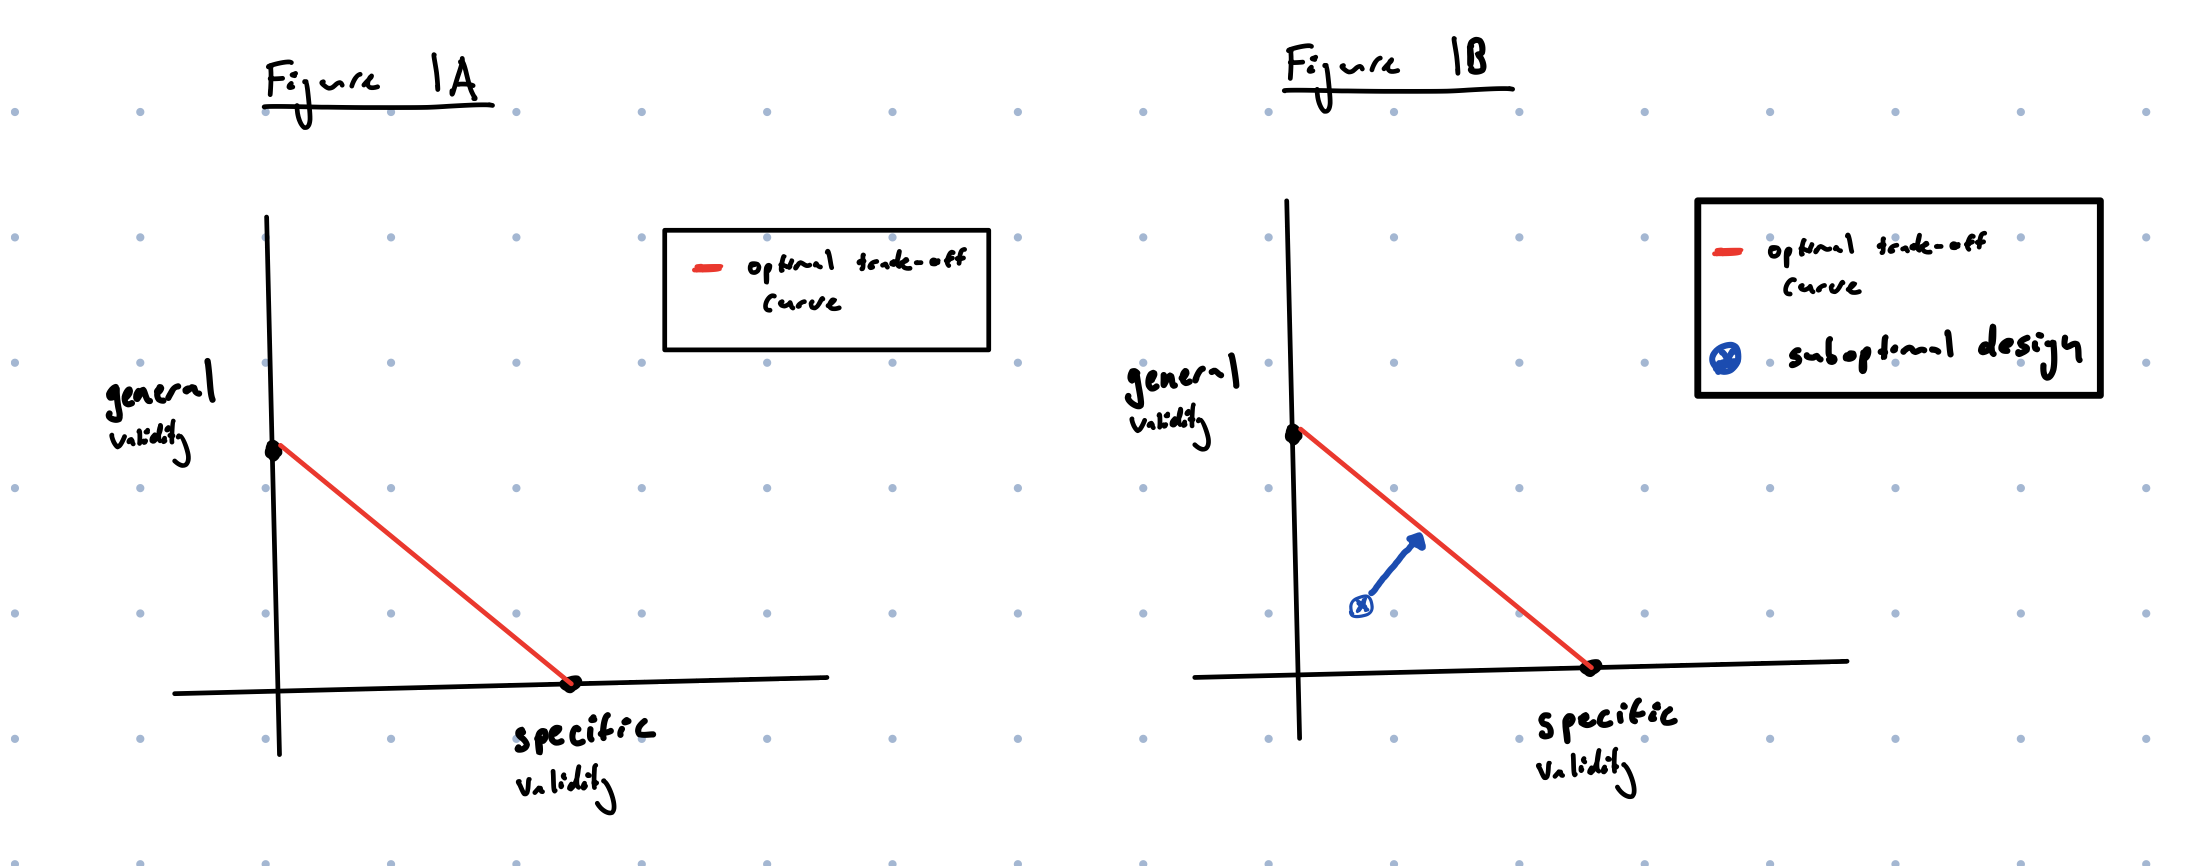
\includegraphics[width=0.9\linewidth]{figures/ch4-optimal-tradeoff-curve.png}
    \label{fig:optimal_tradeoff_curve}
\end{figure}

\par

\vspace{\baselineskip}

\subsection{(Sub)Optimal Approaches}

\vspace{\baselineskip}
At this stage, it’s clear that Monte Carlo based evaluation is a particularly useful method of assessing the performance of causal inference estimators. In the real world, practitioners deal with finite data samples from unknown but complex DGPs. Monte Carlo is capable of evaluating estimators in these settings while theoretical analysis is hard or impossible. It is also clear that Monte Carlo evaluation can vary in validity along two axes - specific and general validity - and that different designs may make (sub)optimal trade-offs between validity on these axes. The analysis which established these two points applied to Monte Carlo evaluation in an abstract sense. This section reviews concrete implementations of Monte Carlo evaluation of causal inference estimators from the literature, analyzing them in light of the axes of validity introduced above. This move toward analyzing concrete implementations brings with it vocabulary which is specific to causal inference. I refer the reader to the theory chapter above for clarification of any unfamiliar terms.\par


\vspace{\baselineskip}
The analysis in this section divides Monte Carlo evaluation methods into two categories based on the underlying design of their DGP: \textit{pure} and \textit{hybrid}. \textit{Pure} methods are further subdivided into purely \textit{synthetic }and \textit{empirical }DGP designs. \textit{Hybrid }designs\ are hybrids because they combine the two pure designs strategies in a single DGP. This is a ‘novel’ ontology introduced to summarize the existing variants of Monte Carlo. All of the designs share the same fundamental structure  - in the sense that the same variables must be sampled so that a causal inference estimator can be evaluated - but exhibit different validity characteristics when judged through the lens of specific and general validity. I proceed by, first, establishing a generic DGP - an abstract representation of the DGP used in all Monte Carlo evaluation methods. I then express the various designs found in the literature in terms of different strategies for the concretizations of this generic DGP, making comparative analysis straightforward. Finally, I analyze the implication of different concretization strategies in terms of the axes of validity from above.\par

\subsubsection{A Generic DGP for the Monte Carlo Evaluation of Causal Inference Estimators}

This sections builds towards a formal specification scheme for the DGPs which underpin Monte Carlo evaluation of causal inference estimators. The scheme is defined in terms of a generic DGP, the functional components of which can then be defined/instantiated to describe a specific, concrete DGP design.\par

First, Table \ref{tbl:var-definitions} below recapitulates the variables over which a causal inference problem-instance is defined and provides the associated dimensionality and  definition. Full explanations for these variables are presented in Chapter \ref{chap:framework} above.\par

\vspace{\baselineskip}

\begin{table}[H]
\begin{tabular}{|p{1in}|p{4in}|}
\hline

$X \in R^{ \left( n, d \right) }$ & $X$ is the covariate matrix that contains measurements of $d$ covariates for a population of $n$ individuals \\ \hline

$T \in \{0, 1\}^n$ & $T$ is the treatment status of the $n$ individuals for a binary treatment \\ \hline

$Y_0 \in R^n$ & $Y_0$ is the outcome under control (absence of treatment) \\ \hline

$Y_1 \in R^n$ & $Y_1$ is the outcome under treatment \\ \hline

$TE \in R^n$ & $TE$ is the individual treatment effect \\ \hline

$Y \in R^n$ & $Y$ is the observed outcome \\ \hline
\end{tabular}

\caption{Variables which define a causal inference problem instance}
\label{tbl:var-definitions}
\end{table}

\vspace{\baselineskip}

The variables in Table \ref{tbl:var-definitions} are related through four generic functions given in Table \ref{tbl:func-definitions}. A concrete Monte Carlo evaluation design can, thus, be fully specified by the concrete instantiation of these four functions.\par


\begin{table}[H]
\begin{tabular}{|p{1.25in}|p{3.75in}|}
\hline

$\rho :  \left(  \right)   \rightarrow R^{ \left( n, d \right) }$ & The \textbf{covariate population sampler} which represents the joint distribution over the  \( d \)  covariates and produces samples of the covariate matrix  \( X. \) Strictly speaking,  \( X \) contains sampled covariate observations for  \( n \) individuals such that a ‘sampled’  \( X \) is constructed by repeatedly sampling the underlying joint distribution over the covariates \\ \hline

$ \Omega :~R^{ \left( n, d \right) }~ \rightarrow R^{n}$ & The \textbf{treatment assignment sampler} which assigns a treatment status  \( T \) to the individuals in  \( X \)  \\ \hline

$\Phi :~R^{ \left( n, d \right) }~ \rightarrow R^{n}$ & The \textbf{outcome sampler} which assigns an outcome under control ( \( Y_{0} \) ) to the individuals in  \( X \) \\ \hline

$ \tau:~R^{ \left( n, d \right) }~ \rightarrow R^{n}$ & The \textbf{treatment effect} \textbf{sampler} which assigns a treatment effect ( \(  \tau \) ) to the individuals in  \( X \) \\ \hline

\end{tabular}

\caption{Functions which generate and relate the variables in a causal inference problem instance}
\label{tbl:func-definitions}
\end{table}

\vspace{\baselineskip}

The complete DGP is then given by the procedure presented in Table \ref{tbl:generic-dgp-definition}. This procedure relates the variables defined in Table \ref{tbl:var-definitions} using the functions defined in Table \ref{tbl:func-definitions}.


\begin{table}[H]
\centering
\begin{tabular}{|l|}
\hline
\textbf{Generic DGP Procedure} \\ \hline

 \( X \leftarrow  \rho  \left(  \right)  \) \\

 \( T \leftarrow  \Omega  \left( X \right)  \) \\

 \( Y_{0} \leftarrow  \Phi  \left( X \right)  \) \\

 \( TE \leftarrow  \tau \left( X \right)  \) \\

 \( Y_{1}~ \leftarrow Y_{0}+ TE \) \\

 \( Y = T \times Y_{1}+  \left( 1-T \right)  \times Y_{0} \) \\
 \hline
\end{tabular}
\caption{The procedure for a Monte Carlo evaluation DGP defined in terms of the variables from Table \ref{tbl:var-definitions} and functions from Table \ref{tbl:func-definitions}}
\end{table}
\label{tbl:generic-dgp-definition}
\vspace{\baselineskip}

Note three facts about this generic DGP:\par

\vspace{\baselineskip}
\begin{itemize}
	\item The designer has a maximum of four degrees of freedom in specifying the DGP. These degrees of freedom correspond to selecting the four functions  \(  \rho ,~ \Omega ,~ \Phi ,~ \tau \) .\par


\vspace{\baselineskip}
	\item This generic DGP provides all of the information required to evaluate a causal inference estimator. The estimator receives  \( \text{X, T, } \) and \( Y \) and produces an estimate of either  \( E \left[ TE  \vert  X \right]  \)  - the conditional treatment effect - or  \( E \left[ TE \right]  \) , the average treatment effect. The ground-truth (sampled) values of  \( TE \) are then be used to evaluate the estimates. \par


\vspace{\baselineskip}
	\item This DGP is constructed to ensure ignorability. Following Dorie et al (2019): Assume  \(  \Phi ,~ \Omega  \)  and  \(  \tau \) are probability distributions, then we have the following factorization as a result of the DGP form above (and specifically as a result of the absence of  \( T \) as an argument to  \(  \Phi ,~ \tau \) ):  \( p \left( Y_{0},~Y_{1}, T  \vert  X \right)  = p \left( Y_{0},~Y_{1} \vert  X \right)  \times p \left( T \vert X \right)  \)  which implies  \(  p \left( Y_{0},~Y_{1} \vert  T, X \right)  = p \left( Y_{0},~Y_{1} \vert ~ X \right)  \)  or  \( Y_{0},~Y_{1} \bigCI T  \vert  X \) . Non-ignorability can be induced by dropping some of the  \( d \)  covariates in  \( X \)  but, by default, it is guaranteed.
\end{itemize}\par


\vspace{\baselineskip}
Taken together, these three facts mean that specifying the four functions is sufficient to generate a causal inference problem-instance. In fact, the minimal level of constraints on the four degrees of freedom means that this generic DGP can be used to specify a concrete DGP design corresponding to any joint distribution which factors in the way outlined above.\par


\vspace{\baselineskip}
Having established this generic DGP, I turn to the idea of concretization strategies. Different strategies for specifying the four base functions - thus concretizing the generic DGP - give rise to the different design categories which were outlined above. There are three mutually-exclusive and exhaustive strategies for concretely specifying a function:\par


\vspace{\baselineskip}
\begin{enumerate}
	\item A function can be manually specified by constructing a mathematical (distribution) function from elementary mathematical building blocks and specifying all the parameters which appear in its definition. This produces functions with known form and parameter values. I will label functions specified in this way as  \( f_{synthetic} \) . \par


\vspace{\baselineskip}
	\item A function can be estimated from empirical data by specifying a fixed functional form and inferring the unknown parameter values. This produces functions with a known form but unknown ground-truth parameters. Functions produced by this strategy will be labeled  \( f_{estimated} \) . \par


\vspace{\baselineskip}
	\item A function can be ‘specified’ to exactly match empirical data. In this case, the mathematical form of the function and any associated parameter values are unknown. This strategy produces functions labeled  \( f_{empirical} \) .
\end{enumerate}\par


\vspace{\baselineskip}
The latter two strategies necessitate access to empirical data from some target DGP. Variables that are sourced empirically for this purpose will be labeled as  \( A_{empirical} \)  where  \( A~ \in  \{ X, T, Y \}  \) (the set of observable variables).\par


\vspace{\baselineskip}
With the generic DGP and the three concretization strategies in mind, I proceed to review and categorize the designs found in the literature.\par

\subsubsection{Pure Designs for Monte Carlo Evaluation}

Pure designs are pure because they rely exclusively on sampling functions of the type  \( f_{synthetic} \)  - in the case of synthetic designs - or  \( f_{empirical} \) - in the case of empirical designs. Below, I outline each of the resultant design approaches and how they tend to appear in the literature.\par


\vspace{\baselineskip}
\paragraph*{Synthetic Monte Carlo Designs}\par


\vspace{\baselineskip}
Synthetic designs rely on hand crafted functions to specify the four degrees of freedom which control the distribution over covariates, treatment, outcome and treatment effect. These designs are common in literature which introduces new estimators designed to tackle specific distributional settings as the manual specification allows careful control over the resultant joint distribution. For recent examples, see Kunzel et al (2018); Johansson, Kallus $\&$  Shalit (2018), Johansson, Shalit $\&$  Sontag (2016). Designs which fit into this class are used extensively in the literature beyond this small sample of recent papers. Khang and Schafer (2007 $\#$ ref) introduce a benchmark based on four independent, normally distributed covariates, a linear outcome with Gaussian noise, a constant treatment effect and a linear expit for the propensity score. Imbalance is created by variable censoring of individuals based on assignment treatment. This benchmark is cited in over eight hundred works at the time of writing, the majority of which use the proposed DGP for evaluating causal inference estimators or use results from analysis of this kind by others. Kallus (2016 $\#$ ref) introduces a similar benchmark which attempts to more accurately model non-linearities present in real data. The benchmark presented is that work is based on two covariates drawn from a uniform distribution, a non-linear propensity score expit and normally distributed outcomes with means derived from the covariates. This benchmark is cited in 10 other works, mostly those applying semi/nonparametric estimators. In both cases, the stated design principle is to create a DGP that is representative of the kinds of data found in practice.\par


\vspace{\baselineskip}
The top left panel of Figure 2 below represents the synthetic design using the function labels and generic DGP defined above. All four degrees of freedom are specified to be synthetic functions and the consequence is a DGP devoid of empirical grounding. The bottom left panel expresses the Khang and Schafer (2007) DGP design as an assignment of the four base functions.\par


\vspace{\baselineskip}
\paragraph*{Empirical Monte Carlo Designs}\par


\vspace{\baselineskip}
In\ contrast to synthetic designs, empirical designs specify the four functional degrees of freedom using real-world data. The challenge is how to do this in a way that still provides access to the treatment effect which is required to evaluate an estimator. Empirical designs overcome this challenge by using data randomized control trials, replacing the control group with non-randomized survey/administrative observations over the same covariates that were observed in the experiment (Huber, 2013 $\#$ ref). The average effect from the randomized control trial provides the ‘ground truth’ target for the average effect estimand. Examples of this design for evaluation include ($\#$ ref) LaLonde (1986), Fraker and Maynard (1987), Friedlander and Robins (1995), Heckman et al (1998), Dehejia and Wahba (1999), Smith and Todd (2005),  Flores and Mitnik (2009) and Jacob et al. (2009).\par


\vspace{\baselineskip}
There are three things about this design worth noting. First, the empirical specification of the functional degrees of freedom means the true distributional setting is not known. Second, and related, the ground truth is itself an estimate rather than a known value. This produces additional uncertainty in the results which come from this evaluation method. Finally, this design can, by default, on evaluate estimators for the average treatment effect. The conditional average treatment effect must be estimated from the data using the very methods which we would like to evaluate using a Monte Carlo benchmark. This means the evaluation of conditional average treatment estimators is impossible under empirical designs of the kind described here.\par


\vspace{\baselineskip}
The top right panel of Figure 2 below represents the empirical design using the function labels and generic DGP defined above. All four degrees of freedom are specified to empirical functions (although some of these are unknown). The consequence is a DGP grounded in empirical data but with an unknown joint distribution over  \( \text{X, T,} \) and  \( Y \) and an unknown values for the true treatment effect and potential outcomes. The bottom left panel expresses the Lalonde (1986) DGP design as an assignment of the four base functions.\par


\vspace{\baselineskip}
There is an obvious concern worth addressing in calling this a Monte Carlo design. The component functions are specified by data rather than sampling functions which means that the DGP cannot be used to generate multiple samples from the joint distribution over the variables. As a result, this method does not provide access to a sampling distribution for the estimand but rather only a single estimate. I believe the Monte Carlo classification is justified for two reasons despite this concern. Firstly, we can conceive of the empirical design as a single sample from some latent DGP which could - in theory - be used produce more samples. This design might be weakened by the small (single) sample size but this doesn’t change the fundamental principle behind its operation. Second, the analysis below will introduce hybrid designs which share common components with the pure empirical design but do allow sampling. In this sense, the pure empirical design can be thought of the extreme (and somewhat degenerate) end of a Monte Carlo design spectrum.\par

\vspace{\baselineskip}


\begin{table}[H]
\begin{tabular}{|p{1in}|p{2in}|p{2.2in}|}
\hline
 & \textbf{Synthetic Monte Carlo} & \textbf{Empirical Monte Carlo} \\ \hline
 
   \textbf{Concretized DGP} & 
   \parbox{2in}{\begin{flalign*}
   &\rho_{synthetic} \leftarrow f_{synthetic}\\ &\Omega_{synthetic} \leftarrow f_{synthetic} \\  &\Phi_{synthetic} \leftarrow f_{synthetic} \\   &\tau_{synthetic} \leftarrow f_{synthetic} \\
   &X \leftarrow  \rho_{synthetic} \left(  \right) \\ 
   &T \leftarrow  \Omega _{synthetic} \left( X \right) \\
   &Y_{0} \leftarrow  \Phi _{synthetic} \left( X \right)\\
   &TE \leftarrow  \tau_{synthetic} \left( X \right) \\
   &Y_{1}~ \leftarrow Y_{0}+ TE   \\
   &Y = T \times Y_{1}+  \left( 1-T \right)  \times Y_{0}
   \end{flalign*}}
   \parbox{2in} & 
   \parbox{2in}{\begin{flalign*}
   & \rho _{empirical} \leftarrow f_{empirical}=X_{empirical}   \\
   & \Omega _{empirical} \leftarrow f_{empirical~}= T_{empirical}   \\
   & \Phi _{empirical} \leftarrow f_{empirical}= ?   \\
   & \tau_{empirical} \leftarrow f_{empirical} = ?   \\
   & X \leftarrow X_{empirical}   \\
   & T \leftarrow T_{empirical}~   \\
   & Y_{0} \leftarrow ?   \\
   & TE \leftarrow ~?   \\
   & Y_{1}~ \leftarrow ?   \\
   & Y = Y_{empirical} 
   \end{flalign*}}
   \parbox{2in} \\
   \\ \hline
   
   \textbf{Example Concretization} &
   \uline{Khang and Schafer (2007)}
   \parbox{2in}{\begin{flalign*}
     & \rho \leftarrow  N \left( X  \vert  0, 1 \right) \\
     & \Omega _{}~ \leftarrow expit ( -X_{1} + 0.5X_{2}  \\
     & ... - 0.25X_{3} - 0.1X_{4} )\\
     & \Phi _{} \leftarrow N ( Y  \vert  210 + 27.4X_{1} \\
     & ... + 13.7 \left( X_{2}+X_{3}+_{}X_{4} \right) , 1 ) \\
     & \tau \leftarrow ~C~ \in R   \\ 
   \end{flalign*}}
   \parbox{2in} \\ &
   \uline{Lalonde (1986)}
   \parbox{2in}{\begin{flalign*}
     & \rho _{} \leftarrow  \{ X_{experiment},~X_{survey} \}  \sim~? \\
     & \Omega _{} \leftarrow ~T_{empirical}~\sim~?  \\
     & \Phi _{} \leftarrow ~? \\
     & \tau_{} \leftarrow ~? \\
   \end{flalign*}}
   \parbox{2in} \\
   \\ \hline
   \textbf{Joint Distribution over Observables} &
   \parbox{2in}{\begin{flalign*}
     & P \left( X, Y, T \right)  \sim \rho  \times  \Omega  \times  \Phi
   \end{flalign*}}
   \parbox{2in} \\ &
   \parbox{2in}{\begin{flalign*}
     & P \left( X, Y, T \right)  \sim~?
   \end{flalign*}}
   \parbox{2in} \\
   \\ \hline
   
   
   
\end{tabular}
\caption{XXX}
\label{tbl:synth-vs-emp-dgp}
\end{table}

\begin{table}[H]
 			\centering
\begin{tabular}{p{0.91in}p{2.7in}p{2.24in}}
\hline
%row no:1
\multicolumn{1}{|p{0.91in}}{} & 
\multicolumn{1}{|p{2.7in}}{\textbf{Synthetic Monte Carlo}} & 
\multicolumn{1}{|p{2.24in}|}{\textbf{Empirical Monte Carlo}} \\
\hhline{---}
%row no:2
\multicolumn{1}{|p{0.91in}}{{\fontsize{9pt}{10.8pt}\selectfont \textbf{Concretized DGP}}} & 
\multicolumn{1}{|p{2.7in}}{ \(  \rho _{synthetic} \leftarrow f_{synthetic}~ \)  \par  \(  \Omega _{synthetic} \leftarrow f_{synthetic} \)  \par  \(  \Phi _{synthetic} \leftarrow f_{synthetic} \)  \par  \(  \tau_{synthetic} \leftarrow f_{synthetic}~ \)  \par  \( X \leftarrow  \rho _{synthetic} \left(  \right)  \)  \par  \( T \leftarrow  \Omega _{synthetic} \left( X \right)  \)  \par  \( Y_{0} \leftarrow  \Phi _{synthetic} \left( X \right)  \)  \par  \( TE \leftarrow  \tau_{synthetic} \left( X \right)  \)  \par  \( Y_{1}~ \leftarrow Y_{0}+ TE \)  \par  \( Y = T \times Y_{1}+  \left( 1-T \right)  \times Y_{0} \)  \par } & 
\multicolumn{1}{|p{2.24in}|}{ \(  \rho _{empirical} \leftarrow f_{empirical}=X_{empirical} \)  \par  \(  \Omega _{empirical} \leftarrow f_{empirical~}= T_{empirical} \)  \par  \(  \Phi _{empirical} \leftarrow f_{empirical}= ? \)  \par  \(  \tau_{empirical} \leftarrow f_{empirical} = ? \)  \par  \( X \leftarrow X_{empirical} \)  \par  \( T \leftarrow T_{empirical}~ \)  \par  \( Y_{0} \leftarrow ? \)  \par  \( TE \leftarrow ~? \)  \par  \( Y_{1}~ \leftarrow ? \)  \par  \( Y = Y_{empirical} \)  \par } \\
\hhline{---}
%row no:3
\multicolumn{1}{|p{0.91in}}{{\fontsize{9pt}{10.8pt}\selectfont \textbf{Example Concretization}}} & 
\multicolumn{1}{|p{2.7in}}{{\fontsize{9pt}{10.8pt}\selectfont \uline{Khang and Schafer (2007)}} \par  \(  \rho _{}~ \leftarrow  N \left( X  \vert  0, 1 \right)  \)  \par  \(  \Omega _{}~ \leftarrow expit \left( -X_{1} + 0.5X_{2} - 0.25X_{3} - 0.1X_{4} \right)  \)  \par  \(  \Phi _{} \leftarrow N \left( Y  \vert  210 + 27.4X_{1} + 13.7 \left( X_{2}+X_{3}+_{}X_{4} \right) , 1 \right)  \)  \par  \(  \tau_{}~ \leftarrow ~C~ \in R \)  \par } & 
\multicolumn{1}{|p{2.24in}|}{{\fontsize{9pt}{10.8pt}\selectfont \uline{Lalonde (1986)}} \par  \(  \rho _{} \leftarrow  \{ X_{experiment},~X_{survey} \}  \sim~? \)  \par  \(  \Omega _{} \leftarrow ~T_{empirical}~\sim~? \)  \par  \(  \Phi _{} \leftarrow ~? \)  \par  \(  \tau_{} \leftarrow ~? \)  \par } \\
\hhline{---}
%row no:4
\multicolumn{1}{|p{0.91in}}{{\fontsize{9pt}{10.8pt}\selectfont \textbf{Joint Distribution over Observables}}} & 
\multicolumn{1}{|p{2.7in}}{ \( P \left( X, Y, T \right)  \sim \rho  \times  \Omega  \times  \Phi  \) } & 
\multicolumn{1}{|p{2.24in}|}{ \( P \left( X, Y, T \right)  \sim~? \) } \\
\hhline{---}

\end{tabular}
 \end{table}


%%%%%%%%%%%%%%%%%%%% Table No: 1 ends here %%%%%%%%%%%%%%%%%%%%


\vspace{\baselineskip}
Figure 2: Synthetic vs Empirical Monte Carlo Designs expressed as concretized versions of the generic DGP along with examples framed in terms of assignments to the four functional degrees of freedom.\par


\vspace{\baselineskip}
\paragraph*{Comparing the Designs}\par


\vspace{\baselineskip}
The framing proposed above clarifies how the theoretical trade-off between specific and general validity manifests in the pure design strategies. Synthetic designs provide granular control of a well-defined distributional setting because all of the component degrees of freedom are set by hand with functions of known form and parameterization. This enables easy testing of estimators across a range of settings, promoting general validity. But, the hand-crafted nature of the function specification raises concerns about the correspondence of the DGP to reality, thereby weakening specific validity. Empirical designs are realistic and correspond to a valid evaluation (with some caveats) of a specific distributional setting (specific validity) but do not allow for easy control of the distributional setting, weakening general validity.\par


\vspace{\baselineskip}
This comparison between the designs, grounded in concretization strategies, provides some insight but is still too abstract. It is unclear what is meant by the ideas of realism and control which appear throughout the paragraph above. Below, I synthesize the work in Paxton (2001), Huber et al (2013) and Dorie et al (2019) to compare the properties of synthetic and empirical designs that contribute to specific and general validity. Many of the points which appear below are implicit or explicit in the analysis above but this complete enumeration will prove useful later when considering hybrid designs which mix the properties of the pure designs.\par


\vspace{\baselineskip}
\textbf{Synthetic designs} tend to have weak specific validity for three reasons which stem from the manual specification of functions:\par


\vspace{\baselineskip}
\begin{itemize}
	\item Unrealistic covariate distributions: the number, type (continuous, categorical, binary) and joint distribution (over the covariates) is often poorly calibrated to the data researchers encounter in practice. It is unlikely that covariates in the real-world are drawn from a multivariate normal distribution.\par


\vspace{\baselineskip}
	\item Unrealistic treatment and outcome functions: the complexity of the functional forms - in terms of interactions, non-linearity etc - is often poorly calibrated to mechanisms likely to be found in the real world. It is unlikely that the treatment policy in the real world is a logistic function with a linear expit.\par


\vspace{\baselineskip}
	\item The potential for specification bias: because covariates and treatment/outcome functions are selected by hand there is the potential for intentional or unintentional bias in the design such that the DGP favors the method being evaluated. This implies DGPs with similar properties would or could lead to worse results. Consider that many researchers may change the DGP specification until their method produces the results they \textit{expect} to see from it under the assumption that their DGP specification, and not their method, is at fault for unexpected results. This would induce the kind of bias described here.
\end{itemize}\par


\vspace{\baselineskip}
However, synthetic designs have three characteristics which counter-balance those above when considering specific validity:\par


\vspace{\baselineskip}
\begin{itemize}
	\item The DGP can be guaranteed to meet the assumptions required for observational causal inference, specifically ignorability and overlap. This avoids false negatives in which an otherwise valid estimator produces poor results as a result of violated assumptions rather than inherent flaws.\par


\vspace{\baselineskip}
	\item The DGP can be used to produce many samples and, therefore, to ensure convergence to a true sampling distributions for the estimand. Further, this provides access to a distribution over performance which is useful for quantifying best and worst case performance.\par


\vspace{\baselineskip}
	\item The DGP provides access to the ground truth of the individual treatment effect and average treatment effect. This precludes the need for additional estimation of the ground truth and means that a wider range of estimators can be evaluated.
\end{itemize}\par


\vspace{\baselineskip}
Moving on to consider general validity, synthetic designs have two properties which make for strong general validity:\par


\vspace{\baselineskip}
\begin{itemize}
	\item The joint distribution over covariates, treatment and outcomes is well-defined and known. This means the performance of the estimator is relative to a known distributional setting.\par


\vspace{\baselineskip}
	\item The distributional setting is controllable such that the estimator can be tested over a range of settings.
\end{itemize}\par


\vspace{\baselineskip}
\textbf{Empirical designs} are effectively polar opposite to synthetic designs when examined in terms of the eight properties above. In order of the points above: They possess inherently realistic covariate distributions and outcome/treatment functions and, by extension, unbiased specification (given that the researcher has no control). However, they do not guarantee that causal inference assumptions are met, do not allow repeat sampling and do not provide access to the ground truth of the average or individual treatment effect without estimation. Further, they use DGPs with an unknown distributional setting and do not allow for researcher control.\par


\vspace{\baselineskip}
Table 2 provides a summary of the eight properties outlined above, which of the two validity axes they affect, and the functional degrees of freedom from the generic DGP which affect each one, and whether each of the two pure designs possesses the (positive) property.\par


\vspace{\baselineskip}


%%%%%%%%%%%%%%%%%%%% Table No: 2 starts here %%%%%%%%%%%%%%%%%%%%


\begin{table}[H]
 			\centering
\begin{tabular}{p{2.31in}p{0.58in}p{0.76in}p{0.64in}p{0.68in}}
\hline
%row no:1
\multicolumn{1}{|p{2.31in}}{\textbf{Property}} & 
\multicolumn{1}{|p{0.58in}}{\textbf{Validity Axis }} & 
\multicolumn{1}{|p{0.76in}}{\textbf{Relevant functional degrees of freedom}} & 
\multicolumn{1}{|p{0.64in}}{\textbf{Synthetic Designs}} & 
\multicolumn{1}{|p{0.68in}|}{\textbf{Empirical Designs}} \\
\hhline{-----}
%row no:2
\multicolumn{1}{|p{2.31in}}{{\fontsize{9pt}{10.8pt}\selectfont Realistic Covariate Distribution}} & 
\multicolumn{1}{|p{0.58in}}{{\fontsize{9pt}{10.8pt}\selectfont Specific}} & 
\multicolumn{1}{|p{0.76in}}{ \(  \rho  \) } & 
\multicolumn{1}{|p{0.64in}}{\cellcolor[HTML]{F4CCCC}{\fontsize{9pt}{10.8pt}\selectfont No}} & 
\multicolumn{1}{|p{0.68in}|}{\cellcolor[HTML]{D9EAD3}{\fontsize{9pt}{10.8pt}\selectfont Yes}} \\
\hhline{-----}
%row no:3
\multicolumn{1}{|p{2.31in}}{{\fontsize{9pt}{10.8pt}\selectfont Realistic Treatment/Outcome Functions}} & 
\multicolumn{1}{|p{0.58in}}{{\fontsize{9pt}{10.8pt}\selectfont Specific}} & 
\multicolumn{1}{|p{0.76in}}{ \(  \Omega ,~ \Phi ,~ \tau \) } & 
\multicolumn{1}{|p{0.64in}}{\cellcolor[HTML]{F4CCCC}{\fontsize{9pt}{10.8pt}\selectfont No}} & 
\multicolumn{1}{|p{0.68in}|}{\cellcolor[HTML]{D9EAD3}{\fontsize{9pt}{10.8pt}\selectfont Yes}} \\
\hhline{-----}
%row no:4
\multicolumn{1}{|p{2.31in}}{{\fontsize{9pt}{10.8pt}\selectfont Guaranteed Unbiased Specification}} & 
\multicolumn{1}{|p{0.58in}}{{\fontsize{9pt}{10.8pt}\selectfont Specific}} & 
\multicolumn{1}{|p{0.76in}}{ \(  \rho ,~ \Omega ,~ \Phi ,~ \tau \) } & 
\multicolumn{1}{|p{0.64in}}{\cellcolor[HTML]{F4CCCC}{\fontsize{9pt}{10.8pt}\selectfont No}} & 
\multicolumn{1}{|p{0.68in}|}{\cellcolor[HTML]{D9EAD3}{\fontsize{9pt}{10.8pt}\selectfont Yes}} \\
\hhline{-----}
%row no:5
\multicolumn{1}{|p{2.31in}}{{\fontsize{9pt}{10.8pt}\selectfont Access to Ground Truth}} & 
\multicolumn{1}{|p{0.58in}}{{\fontsize{9pt}{10.8pt}\selectfont Specific}} & 
\multicolumn{1}{|p{0.76in}}{ \(  \Phi ,~ \tau \) } & 
\multicolumn{1}{|p{0.64in}}{\cellcolor[HTML]{D9EAD3}{\fontsize{9pt}{10.8pt}\selectfont Yes}} & 
\multicolumn{1}{|p{0.68in}|}{\cellcolor[HTML]{F4CCCC}{\fontsize{9pt}{10.8pt}\selectfont No}} \\
\hhline{-----}
%row no:6
\multicolumn{1}{|p{2.31in}}{{\fontsize{9pt}{10.8pt}\selectfont Guaranteed to Obey Causal Assumptions}} & 
\multicolumn{1}{|p{0.58in}}{{\fontsize{9pt}{10.8pt}\selectfont Specific}} & 
\multicolumn{1}{|p{0.76in}}{ \(  \Omega ,~ \Phi ,~ \tau \) } & 
\multicolumn{1}{|p{0.64in}}{\cellcolor[HTML]{D9EAD3}{\fontsize{9pt}{10.8pt}\selectfont Yes}} & 
\multicolumn{1}{|p{0.68in}|}{\cellcolor[HTML]{F4CCCC}{\fontsize{9pt}{10.8pt}\selectfont No}} \\
\hhline{-----}
%row no:7
\multicolumn{1}{|p{2.31in}}{{\fontsize{9pt}{10.8pt}\selectfont Allows Repeat Sampling}} & 
\multicolumn{1}{|p{0.58in}}{{\fontsize{9pt}{10.8pt}\selectfont Specific}} & 
\multicolumn{1}{|p{0.76in}}{ \(  \rho ,~ \Omega ,~ \Phi ,~ \tau \) } & 
\multicolumn{1}{|p{0.64in}}{\cellcolor[HTML]{D9EAD3}{\fontsize{9pt}{10.8pt}\selectfont Yes}} & 
\multicolumn{1}{|p{0.68in}|}{\cellcolor[HTML]{F4CCCC}{\fontsize{9pt}{10.8pt}\selectfont No}} \\
\hhline{-----}
%row no:8
\multicolumn{1}{|p{2.31in}}{{\fontsize{9pt}{10.8pt}\selectfont Known Distributional Setting}} & 
\multicolumn{1}{|p{0.58in}}{{\fontsize{9pt}{10.8pt}\selectfont General}} & 
\multicolumn{1}{|p{0.76in}}{ \(  \rho ,~ \Omega ,~ \Phi ,~ \tau \) } & 
\multicolumn{1}{|p{0.64in}}{\cellcolor[HTML]{D9EAD3}{\fontsize{9pt}{10.8pt}\selectfont Yes}} & 
\multicolumn{1}{|p{0.68in}|}{\cellcolor[HTML]{F4CCCC}{\fontsize{9pt}{10.8pt}\selectfont No}} \\
\hhline{-----}
%row no:9
\multicolumn{1}{|p{2.31in}}{{\fontsize{9pt}{10.8pt}\selectfont Controllable Distributional Setting}} & 
\multicolumn{1}{|p{0.58in}}{{\fontsize{9pt}{10.8pt}\selectfont General}} & 
\multicolumn{1}{|p{0.76in}}{ \(  \rho ,~ \Omega ,~ \Phi ,~ \tau \) } & 
\multicolumn{1}{|p{0.64in}}{\cellcolor[HTML]{D9EAD3}{\fontsize{9pt}{10.8pt}\selectfont Yes}} & 
\multicolumn{1}{|p{0.68in}|}{\cellcolor[HTML]{F4CCCC}{\fontsize{9pt}{10.8pt}\selectfont No}} \\
\hhline{-----}

\end{tabular}
 \end{table}


%%%%%%%%%%%%%%%%%%%% Table No: 2 ends here %%%%%%%%%%%%%%%%%%%%


\vspace{\baselineskip}
Table 2: the eight properties of Monte Carlo designs which affect specific and general validity of evaluation along with the functional degrees of freedom which impact this property.\par


\vspace{\baselineskip}
The analysis above establishes a more granular understanding of the properties of the two pure designs which produce the differences in their specific and general validity. It is clear that these two designs are polar opposites but this does not necessarily mean that they are suboptimal in terms of the trade-off between specific and general validity. If one could not do better in one without sacrificing the other, then these two designs would represent a (discrete) optimal frontier with researchers being forced to choose one or the other depending on their needs. Fortunately, this is not the case.

\subsubsection{Hybrid Designs for Monte Carlo Evaluation}

Hybrid designs combine the concretization strategies from synthetic and empirical designs to produce a Monte Carlo evaluation method with more of the desirable properties enumerated above. The unifying principle behind hybrid designs is the maximal use of data to inform specification of the DGP - to improve realism and specific validity - while maintaining the control required to allow general validity.\par


\vspace{\baselineskip}
The earliest examples of thought in the direction of blending synthetic and empirical designs appear in Abadie and Imbens (2002 $\#$ ref) and Diamond and Sekhon (2008). Both papers use DGPs designed to mimic the data in Lalonde (1986) but both use synthetic, simplified covariate sampling and hand-crafted treatment/outcome functions which are ‘inspired’ by the data but not directly informed by it.\par


\vspace{\baselineskip}
Huber et al (2013) formalize this idea and introduce what they call \textit{Empirical Monte Carlo }(EMC). The context for the introduction of their method is instructive. Their paper attempts to resolve a disagreement between Frolich (2004) and Busso et al (2009), both of whom evaluate the same set of propensity-score based estimators using synthetic Monte Carlo but find quite different results. Huber et al (2013) points out that both papers use DGPS with poor specific validity as a result of arbitrary synthetic design. This inspires the design of a method which uses a $``$DGP not entirely [built] on relations specified by the researcher, but [one which] exploits real data as much as possible instead, [using] observed outcomes and covariates instead of simulated ones as well as an observed selection process$"$ . The authors propose the following design: They define a population of observations as a dataset covering all German nationals with social insurance in the years between 1990 and 2006 (millions of observations). The treatment is participation in any employment assistance program during the observed period and the outcome is the employment status in the 36 months following participation. EMC then involves four steps: \par


\vspace{\baselineskip}
\begin{enumerate}
	\item A propensity score model is estimated based on the entire population using a logistic regression with a linear expit.\par

	\item A random sample of the non-treated individuals is drawn from the population. This means the observed outcome - with an unknown functional relation to the covariates - serves as the value  \( Y_{0} \) .\par

	\item Each individual is assigned a treatment status based on a draw from a Bernoulli distribution parameterized by the propensity score for the individual under the model from step 1.\par

	\item Each individual is subjected to a ‘placebo’ treatment to construct  \( Y_{1}. \) This is treatment with a constant, zero treatment effect.\par

	\item Steps 2 through 4 are repeated for multiple samples.
\end{enumerate}\par


\vspace{\baselineskip}
Figure 3 expresses this design using the generic DGP and functional building blocks from above.\par


\vspace{\baselineskip}


%%%%%%%%%%%%%%%%%%%% Table No: 3 starts here %%%%%%%%%%%%%%%%%%%%


\begin{table}[H]
 			\centering
\begin{tabular}{p{3.14in}}
\hline
%row no:1
\multicolumn{1}{|p{3.14in}|}{\textbf{Empirical Monte Carlo - Huber et al (2013)} \par  \(  \rho _{} \leftarrow f_{empirical}~ \)  \par  \(  \Omega _{} \leftarrow f_{estimate} \)  \par  \(  \Phi _{} \leftarrow f_{empirical} \)  \par  \(  \tau_{} \leftarrow f_{synthetic}~ \)  \par  \( X \leftarrow X_{empirical} \)  \par  \( T \leftarrow LogisticFit \left(  T_{empirical}\simX_{empirical} \right)  \)  \par  \( Y_{0} \leftarrow Y_{empirical} \)  \par  \( TE \leftarrow 0 \)  \par  \( Y_{1}~ \leftarrow Y_{0}+ TE \)  \par  \( Y = T \times Y_{1}+  \left( 1-T \right)  \times Y_{0} \)  \par } \\
\hhline{-}

\end{tabular}
 \end{table}


%%%%%%%%%%%%%%%%%%%% Table No: 3 ends here %%%%%%%%%%%%%%%%%%%%


\vspace{\baselineskip}
Figure 3: Concretization of the generic DGP under the design of Huber et al (2013)\par


\vspace{\baselineskip}
Analyzing the assignment of the functional degrees of freedom from Figure 3 in light of Table 2 makes analyzing the validity properties of this design relatively straightforward. These are listed below with a summary given in Table 3. It is clear from these properties that hybrid designs are promising - the use of data provides realism while the simulated components of the treatment and outcome provide access to ground truth and ensure assumptions are obeyed. However, as is evident from the analysis below, the EMC design provides only partial conformance to some of the desirable properties of validity.\par


\vspace{\baselineskip}
\begin{itemize}
	\item \textbf{Realistic Covariate Distribution - Yes: }The use of observed covariates means the covariate distribution is realistic (in the specific domain of labour data).\par


\vspace{\baselineskip}
	\item \textbf{Realistic Treatment/Outcome Functions - Partial: }The use of the observed outcome mechanism means this too is realistic. However, the treatment assignment and treatment effect are both hand crafted and too simplistic.\par


\vspace{\baselineskip}
	\item \textbf{Guaranteed unbiased specification - No: }The hand selection of the two functions above means there is potential for researcher bias (which holds even if more complex functions are chosen).\par


\vspace{\baselineskip}
	\item \textbf{Access to ground truth - Yes: }the simulated treatment means the ground truth is known at the individual and average effect level.\par


\vspace{\baselineskip}
	\item \textbf{Guaranteed to meet causal assumptions - Yes: }the treatment assignment mechanism is known to include only the observed covariates so we have selection on observables and therefore ignorability. The authors also include an offset in the treatment assignment expit to ensure that the probability of treatment is bounded away from 0 and 1, meaning there is overlap. So both important causal assumptions are met.\par


\vspace{\baselineskip}
	\item \textbf{Allows repeat sampling - Yes: }the large population of observations allows repeat samping as in a synthetic Monte Carlo design:\par


\vspace{\baselineskip}
	\item \textbf{Known distributional setting - Weak: }the joint distribution over the covariates and the outcome is unknown. The treatment assignment mechanism is known.\par


\vspace{\baselineskip}
	\item \textbf{Controllable distributional setting - Weak: }the treatment assignment mechanism can be altered but the joint distribution over the covariates and the outcome mechanism is fixed by the data.
\end{itemize}\par


\vspace{\baselineskip}
Knaus et al (2018) build on EMC. They use a very similar dataset as Huber et al (2013) - but covering Swiss administrative data on labour and employment rather than German. They also share the same logistic estimation for the treatment assignment. But, unlike Huber et al, they specify a non-zero, non-constant treatment effect mechanism. This is specified synthetically rather than estimated because $``$estimation may favor [functionally] similar estimators under investigation$"$ . It is unclear why the authors are concerned about this problem in outcome mechanism but are ok with fixed functional form estimation in the treatment assignment mechanism. This paper is designed to test methods which infer individual treatment effects, so the authors specify the treatment effect mechanism with the goal of $``$making disambiguating selection and treatment effect heterogeneity hard$"$ . To this end, they include the propensity score in the synthetic treatment effect and apply a highly non-linear transform and add random noise. The treatment effect from this function is added to the observed  \( Y_{0} \) outcome (much like in EMC, only non-treated individuals are selected into samples). In addition to the synthetic treatment effect, the authors parameterize the population sampler, treatment assignment mechanism and treatment effect function to generate 24 datasets with different sample sizes, treatment effect magnitude, treatment effect heterogeneity, and counts of treated vs control individuals.\par


\vspace{\baselineskip}

\vspace{\baselineskip}


%%%%%%%%%%%%%%%%%%%% Table No: 4 starts here %%%%%%%%%%%%%%%%%%%%


\begin{table}[H]
 			\centering
\begin{tabular}{p{3.14in}}
\hline
%row no:1
\multicolumn{1}{|p{3.14in}|}{\textbf{Knaus et al (2018)} \par  \(  \rho _{} \leftarrow f_{empirical}~ \)  \par  \(  \Omega _{} \leftarrow f_{estimate} \)  \par  \(  \Phi _{} \leftarrow f_{empirical} \)  \par  \(  \tau_{} \leftarrow f_{synthetic}~ \)  \par  \( X \leftarrow X_{empirical} \)  \par  \( T \leftarrow LogisticFit \left(  T_{empirical}\simX_{empirical} \right)  \)  \par  \( Y_{0} \leftarrow Y_{empirical} \)  \par  \( TE \leftarrow f_{synthetic} \)  \par  \( Y_{1}~ \leftarrow Y_{0}+ TE \)  \par  \( Y = T \times Y_{1}+  \left( 1-T \right)  \times Y_{0} \)  \par } \\
\hhline{-}

\end{tabular}
 \end{table}


%%%%%%%%%%%%%%%%%%%% Table No: 4 ends here %%%%%%%%%%%%%%%%%%%%


\vspace{\baselineskip}
Figure 4: Concretization of the generic DGP under the design of Huber et al (2013)\par


\vspace{\baselineskip}
The concretized DGP is given in Figure 4. This figure makes the similarity with Huber et al obvious. But the changes do represent a moderate improvement over EMC when examining the validity properties. The outcome mechanism is arguably more realistic as a result of the complex synthetic treatment effect function combined with the empirical control outcome. But, the synthetic component of the specification opens this design to the same criticisms of realism and potential bias as any other synthetic design. The primary contribution of these authors is the parameterization of the functions to generate datasets with different, well-defined distributional settings. This allows the evaluation of estimators over a partial subspace of all possible distributional settings. These changes are reflected in the 5th column of Table 3 which upgrades the known and controllable distributional setting properties from weak under EMC to partial under Knaus et al.\par


\vspace{\baselineskip}
The two approaches analyzed above use an empirical covariate population and empirical outcome with an estimated treatment assignment mechanism. There is a loosely analogous set of designs which use an empirical treatment and specify a synthetic outcome. Hill (2011) develops a method to test their new causal estimator based on non-parametric Bayesian regression. The proposed method uses experimental data from the Infant Health and Development Program (IHDP) - a $``$randomized experiment which targeted low birth-weight, premature infants and provided the treatment group with high-quality individual care$"$  (Brooks-Gunn, Liaw, Klebanov, 1991 $\#$ ref). Per Hill (2011), using an experimental dataset guarantees overlap (and balance) in the covariate distributions and simulating the outcome using only the observed covariates ensures ignorability. The outcome mechanism (the outcome function  \(  \Phi  \) and treatment effect function  \(  \tau \) ) are specified by hand - the author chooses two conditions, one linear outcome and constant treatment effect and one non-linear outcome with heterogenous treatment effect. Starting from the position of balanced covariate distribution allows the author to induce imbalance by non-randomly censoring individuals from the treat/control group. This is the first instance of an intentional specification of the level of balance.\par


\vspace{\baselineskip}
The concretization of the generic DGP proposed by hill is summarized in Figure 5. Ultimately, as a result of the parallel between simulating outcome and treatment, this method has very similar validity properties to those analyzed above. Unlike the methods in Huber et al (2013) and Knaus et al (2018), the simulated non-treatment outcome provides greater control over the distribution of outcomes and the experimental datasets allows for the easy control of balance (although a similar censoring method could be applied to non-experimental data). This means the method has arguably better definition and control of the distributional setting but this control is still worse than under purely synthetic treatment assignment and outcome mechanisms.\par


\vspace{\baselineskip}


%%%%%%%%%%%%%%%%%%%% Table No: 5 starts here %%%%%%%%%%%%%%%%%%%%


\begin{table}[H]
 			\centering
\begin{tabular}{p{3.14in}}
\hline
%row no:1
\multicolumn{1}{|p{3.14in}|}{\textbf{Hill (2011)} \par  \(  \rho _{} \leftarrow f_{empirical}~ \)  \par  \(  \Omega _{} \leftarrow f_{empirical} \)  \par  \(  \Phi _{} \leftarrow f_{synthetic} \)  \par  \(  \tau_{} \leftarrow f_{synthetic}~ \)  \par  \( X \leftarrow X_{empirical} \)  \par  \( T \leftarrow T_{empirical} \)  \par  \( Y_{0} \leftarrow f_{synthetic} \)  \par  \( TE \leftarrow f_{synthetic} \)  \par  \( Y_{1}~ \leftarrow Y_{0}+ TE \)  \par  \( Y = T \times Y_{1}+  \left( 1-T \right)  \times Y_{0} \)  \par } \\
\hhline{-}

\end{tabular}
 \end{table}


%%%%%%%%%%%%%%%%%%%% Table No: 5 ends here %%%%%%%%%%%%%%%%%%%%


\vspace{\baselineskip}
Figure 5: Concretization of the generic DGP under the design of Hill (2011)\par


\vspace{\baselineskip}
Two papers iterate on the design proposed by Hill (2011) but change the specification of the outcome and treatment effect functions in order to improve the realism of the synthetic outcome and reduce the potential for bias. Wendling (2019 $\#$ ref) uses four experimental datasets from the medical field but, instead of manually specifying the outcome and treatment effect functions, estimates these using neural networks. This technically avoids the need to specify a functional form because neural networks can represent an arbitrary set of functional forms. This is a move back toward the estimation used in EMC with  \(  \Phi _{} \leftarrow f_{estimated} \)  and  \(  \tau_{} \leftarrow f_{estimated}~ \) . While this may more accurately model the true outcome function, the estimation method could still favor specific estimators - for example those based on neural networks which will more naturally recover the same estimated function from the same data. It also gives up on control over the outcome aspect of the distributional setting because it is not clear what level of interaction/non-linearity is represented by the estimated functions nor how to change these functions to change the level of these aspects of the distribution. The first point results in improved realism of the outcome/treatment but no change to the Guaranteed Unbiased Specification property. The second point results in worsened scores on Known and Controllable distributional setting - see Table 3.\par


\vspace{\baselineskip}
Kern et al (2016 $\#$ ref) pursue a different approach - they specify the outcome and treatment effect functions manually but use a $``$saturated parametric model$"$  with some desired level of nonlinearity and interaction. This means that, for example, all covariates may appear in both linear and quadratic form as well as in every possible (pairwise) interaction with lower/higher powers and interaction levels possible. The motivation for this is to create a principled approach for building complex functions with desired properties but without allowing the function to be hand crafted with arbitrary form and/or modified to produce desired results. This moves towards a design that allows for control over the outcome mechanism while also partially mitigating specification bias. Note that the the full saturation is itself fairly arbitrary (although it is closed to respecification in order to achieve desired results). On balance, the result of this change is a design which appears to have some degree of positive across-the-board ‘performance’ when assessed on the properties of validity - see Table 3. This is not a claim to formal superiority but rather an indication of a promising design direction.\par


\vspace{\baselineskip}


%%%%%%%%%%%%%%%%%%%% Table No: 6 starts here %%%%%%%%%%%%%%%%%%%%


\begin{table}[H]
 			\centering
\begin{tabular}{p{0.78in}p{0.57in}p{0.52in}p{-0.02in}p{0.51in}p{0.53in}p{0.51in}p{0.54in}p{0.52in}}
\hline
%row no:1
\multicolumn{1}{|p{0.78in}}{} & 
\multicolumn{2}{|p{\dimexpr1.09in+2\tabcolsep\relax}}{\Centering {\fontsize{9pt}{10.8pt}\selectfont \textbf{Pure Designs}}} & 
\multicolumn{1}{|p{-0.02in}}{\cellcolor[HTML]{000000}} & 
\multicolumn{5}{|p{\dimexpr2.61in+8\tabcolsep\relax}|}{\Centering {\fontsize{9pt}{10.8pt}\selectfont \textbf{Hybrid Designs}}} \\
\hhline{---------}
%row no:2
\multicolumn{1}{|p{0.78in}}{{\fontsize{9pt}{10.8pt}\selectfont \textbf{Property}}} & 
\multicolumn{1}{|p{0.57in}}{{\fontsize{9pt}{10.8pt}\selectfont \textbf{Synthetic Designs}}} & 
\multicolumn{1}{|p{0.52in}}{{\fontsize{9pt}{10.8pt}\selectfont \textbf{Empirical Designs}}} & 
\multicolumn{1}{|p{-0.02in}}{\cellcolor[HTML]{000000}} & 
\multicolumn{1}{|p{0.51in}}{{\fontsize{9pt}{10.8pt}\selectfont \textbf{Huber et al (2013)}}} & 
\multicolumn{1}{|p{0.53in}}{{\fontsize{9pt}{10.8pt}\selectfont \textbf{Knaus et al (2018)}}} & 
\multicolumn{1}{|p{0.51in}}{{\fontsize{9pt}{10.8pt}\selectfont \textbf{Hill (2011)}}} & 
\multicolumn{1}{|p{0.54in}}{{\fontsize{9pt}{10.8pt}\selectfont \textbf{Wendling (2019)}}} & 
\multicolumn{1}{|p{0.52in}|}{{\fontsize{9pt}{10.8pt}\selectfont \textbf{Kern et al (2016)}}} \\
\hhline{---------}
%row no:3
\multicolumn{1}{|p{0.78in}}{{\fontsize{9pt}{10.8pt}\selectfont Realistic Covariate Distribution}} & 
\multicolumn{1}{|p{0.57in}}{\cellcolor[HTML]{F4CCCC}{\fontsize{9pt}{10.8pt}\selectfont No}} & 
\multicolumn{1}{|p{0.52in}}{\cellcolor[HTML]{D9EAD3}{\fontsize{9pt}{10.8pt}\selectfont Yes}} & 
\multicolumn{1}{|p{-0.02in}}{\cellcolor[HTML]{000000}} & 
\multicolumn{1}{|p{0.51in}}{\cellcolor[HTML]{D9EAD3}{\fontsize{9pt}{10.8pt}\selectfont Yes}} & 
\multicolumn{1}{|p{0.53in}}{\cellcolor[HTML]{D9EAD3}{\fontsize{9pt}{10.8pt}\selectfont Yes}} & 
\multicolumn{1}{|p{0.51in}}{\cellcolor[HTML]{D9EAD3}{\fontsize{9pt}{10.8pt}\selectfont Yes}} & 
\multicolumn{1}{|p{0.54in}}{\cellcolor[HTML]{D9EAD3}{\fontsize{9pt}{10.8pt}\selectfont Yes}} & 
\multicolumn{1}{|p{0.52in}|}{\cellcolor[HTML]{D9EAD3}{\fontsize{9pt}{10.8pt}\selectfont Yes}} \\
\hhline{---------}
%row no:4
\multicolumn{1}{|p{0.78in}}{{\fontsize{9pt}{10.8pt}\selectfont Realistic Treatment/Outcome Functions}} & 
\multicolumn{1}{|p{0.57in}}{\cellcolor[HTML]{F4CCCC}{\fontsize{9pt}{10.8pt}\selectfont No}} & 
\multicolumn{1}{|p{0.52in}}{\cellcolor[HTML]{D9EAD3}{\fontsize{9pt}{10.8pt}\selectfont Yes}} & 
\multicolumn{1}{|p{-0.02in}}{\cellcolor[HTML]{000000}} & 
\multicolumn{1}{|p{0.51in}}{\cellcolor[HTML]{FFF2CC}{\fontsize{9pt}{10.8pt}\selectfont Partial}} & 
\multicolumn{1}{|p{0.53in}}{\cellcolor[HTML]{FFF2CC}{\fontsize{9pt}{10.8pt}\selectfont Partial}} & 
\multicolumn{1}{|p{0.51in}}{\cellcolor[HTML]{FFF2CC}{\fontsize{9pt}{10.8pt}\selectfont Partial}} & 
\multicolumn{1}{|p{0.54in}}{\cellcolor[HTML]{FFF2CC}{\fontsize{9pt}{10.8pt}\selectfont Partial but strong\footnote{ Due to non-parametric neural network estimation of outcome function and empirical treatment assignment. }}} & 
\multicolumn{1}{|p{0.52in}|}{\cellcolor[HTML]{FFF2CC}{\fontsize{9pt}{10.8pt}\selectfont Partial}} \\
\hhline{---------}
%row no:5
\multicolumn{1}{|p{0.78in}}{{\fontsize{9pt}{10.8pt}\selectfont Guaranteed Unbiased Specification}} & 
\multicolumn{1}{|p{0.57in}}{\cellcolor[HTML]{F4CCCC}{\fontsize{9pt}{10.8pt}\selectfont No}} & 
\multicolumn{1}{|p{0.52in}}{\cellcolor[HTML]{D9EAD3}{\fontsize{9pt}{10.8pt}\selectfont Yes}} & 
\multicolumn{1}{|p{-0.02in}}{\cellcolor[HTML]{000000}} & 
\multicolumn{1}{|p{0.51in}}{\cellcolor[HTML]{F4CCCC}{\fontsize{9pt}{10.8pt}\selectfont No}} & 
\multicolumn{1}{|p{0.53in}}{\cellcolor[HTML]{F4CCCC}{\fontsize{9pt}{10.8pt}\selectfont No}} & 
\multicolumn{1}{|p{0.51in}}{\cellcolor[HTML]{F4CCCC}{\fontsize{9pt}{10.8pt}\selectfont No}} & 
\multicolumn{1}{|p{0.54in}}{\cellcolor[HTML]{F4CCCC}{\fontsize{9pt}{10.8pt}\selectfont No}} & 
\multicolumn{1}{|p{0.52in}|}{\cellcolor[HTML]{FFF2CC}{\fontsize{9pt}{10.8pt}\selectfont Partial}} \\
\hhline{---------}
%row no:6
\multicolumn{1}{|p{0.78in}}{{\fontsize{9pt}{10.8pt}\selectfont Access to Ground Truth}} & 
\multicolumn{1}{|p{0.57in}}{\cellcolor[HTML]{D9EAD3}{\fontsize{9pt}{10.8pt}\selectfont Yes}} & 
\multicolumn{1}{|p{0.52in}}{\cellcolor[HTML]{F4CCCC}{\fontsize{9pt}{10.8pt}\selectfont No}} & 
\multicolumn{1}{|p{-0.02in}}{\cellcolor[HTML]{000000}} & 
\multicolumn{1}{|p{0.51in}}{\cellcolor[HTML]{D9EAD3}{\fontsize{9pt}{10.8pt}\selectfont Yes}} & 
\multicolumn{1}{|p{0.53in}}{\cellcolor[HTML]{D9EAD3}{\fontsize{9pt}{10.8pt}\selectfont Yes}} & 
\multicolumn{1}{|p{0.51in}}{\cellcolor[HTML]{D9EAD3}{\fontsize{9pt}{10.8pt}\selectfont Yes}} & 
\multicolumn{1}{|p{0.54in}}{\cellcolor[HTML]{D9EAD3}{\fontsize{9pt}{10.8pt}\selectfont Yes}} & 
\multicolumn{1}{|p{0.52in}|}{\cellcolor[HTML]{D9EAD3}{\fontsize{9pt}{10.8pt}\selectfont Yes}} \\
\hhline{---------}
%row no:7
\multicolumn{1}{|p{0.78in}}{{\fontsize{9pt}{10.8pt}\selectfont Guaranteed to Obey Causal Assumptions}} & 
\multicolumn{1}{|p{0.57in}}{\cellcolor[HTML]{D9EAD3}{\fontsize{9pt}{10.8pt}\selectfont Yes}} & 
\multicolumn{1}{|p{0.52in}}{\cellcolor[HTML]{F4CCCC}{\fontsize{9pt}{10.8pt}\selectfont No}} & 
\multicolumn{1}{|p{-0.02in}}{\cellcolor[HTML]{000000}} & 
\multicolumn{1}{|p{0.51in}}{\cellcolor[HTML]{D9EAD3}{\fontsize{9pt}{10.8pt}\selectfont Yes}} & 
\multicolumn{1}{|p{0.53in}}{\cellcolor[HTML]{D9EAD3}{\fontsize{9pt}{10.8pt}\selectfont Yes}} & 
\multicolumn{1}{|p{0.51in}}{\cellcolor[HTML]{D9EAD3}{\fontsize{9pt}{10.8pt}\selectfont Yes}} & 
\multicolumn{1}{|p{0.54in}}{\cellcolor[HTML]{D9EAD3}{\fontsize{9pt}{10.8pt}\selectfont Yes}} & 
\multicolumn{1}{|p{0.52in}|}{\cellcolor[HTML]{D9EAD3}{\fontsize{9pt}{10.8pt}\selectfont Yes}} \\
\hhline{---------}
%row no:8
\multicolumn{1}{|p{0.78in}}{{\fontsize{9pt}{10.8pt}\selectfont Allows Repeat Sampling}} & 
\multicolumn{1}{|p{0.57in}}{\cellcolor[HTML]{D9EAD3}{\fontsize{9pt}{10.8pt}\selectfont Yes}} & 
\multicolumn{1}{|p{0.52in}}{\cellcolor[HTML]{F4CCCC}{\fontsize{9pt}{10.8pt}\selectfont No}} & 
\multicolumn{1}{|p{-0.02in}}{\cellcolor[HTML]{000000}} & 
\multicolumn{1}{|p{0.51in}}{\cellcolor[HTML]{D9EAD3}{\fontsize{9pt}{10.8pt}\selectfont Yes}} & 
\multicolumn{1}{|p{0.53in}}{\cellcolor[HTML]{D9EAD3}{\fontsize{9pt}{10.8pt}\selectfont Yes}} & 
\multicolumn{1}{|p{0.51in}}{\cellcolor[HTML]{D9EAD3}{\fontsize{9pt}{10.8pt}\selectfont Yes}} & 
\multicolumn{1}{|p{0.54in}}{\cellcolor[HTML]{D9EAD3}{\fontsize{9pt}{10.8pt}\selectfont Yes}} & 
\multicolumn{1}{|p{0.52in}|}{\cellcolor[HTML]{D9EAD3}{\fontsize{9pt}{10.8pt}\selectfont Yes}} \\
\hhline{---------}
%row no:9
\multicolumn{1}{|p{0.78in}}{{\fontsize{9pt}{10.8pt}\selectfont Known Distributional Setting}} & 
\multicolumn{1}{|p{0.57in}}{\cellcolor[HTML]{D9EAD3}{\fontsize{9pt}{10.8pt}\selectfont Yes}} & 
\multicolumn{1}{|p{0.52in}}{\cellcolor[HTML]{F4CCCC}{\fontsize{9pt}{10.8pt}\selectfont No}} & 
\multicolumn{1}{|p{-0.02in}}{\cellcolor[HTML]{000000}} & 
\multicolumn{1}{|p{0.51in}}{\cellcolor[HTML]{F9CB9C}{\fontsize{9pt}{10.8pt}\selectfont Weak}} & 
\multicolumn{1}{|p{0.53in}}{\cellcolor[HTML]{FFF2CC}{\fontsize{9pt}{10.8pt}\selectfont Partial}} & 
\multicolumn{1}{|p{0.51in}}{\cellcolor[HTML]{FFF2CC}{\fontsize{9pt}{10.8pt}\selectfont Partial}} & 
\multicolumn{1}{|p{0.54in}}{\cellcolor[HTML]{F9CB9C}{\fontsize{9pt}{10.8pt}\selectfont Weak}} & 
\multicolumn{1}{|p{0.52in}|}{\cellcolor[HTML]{FFF2CC}{\fontsize{9pt}{10.8pt}\selectfont Partial}} \\
\hhline{---------}
%row no:10
\multicolumn{1}{|p{0.78in}}{{\fontsize{9pt}{10.8pt}\selectfont Controllable Distributional Setting}} & 
\multicolumn{1}{|p{0.57in}}{\cellcolor[HTML]{D9EAD3}{\fontsize{9pt}{10.8pt}\selectfont Yes}} & 
\multicolumn{1}{|p{0.52in}}{\cellcolor[HTML]{F4CCCC}{\fontsize{9pt}{10.8pt}\selectfont No}} & 
\multicolumn{1}{|p{-0.02in}}{\cellcolor[HTML]{000000}} & 
\multicolumn{1}{|p{0.51in}}{\cellcolor[HTML]{F9CB9C}{\fontsize{9pt}{10.8pt}\selectfont Weak}} & 
\multicolumn{1}{|p{0.53in}}{\cellcolor[HTML]{FFF2CC}{\fontsize{9pt}{10.8pt}\selectfont Partial}} & 
\multicolumn{1}{|p{0.51in}}{\cellcolor[HTML]{FFF2CC}{\fontsize{9pt}{10.8pt}\selectfont Partial}} & 
\multicolumn{1}{|p{0.54in}}{\cellcolor[HTML]{F9CB9C}{\fontsize{9pt}{10.8pt}\selectfont Weak}} & 
\multicolumn{1}{|p{0.52in}|}{\cellcolor[HTML]{FFF2CC}{\fontsize{9pt}{10.8pt}\selectfont Partial}} \\
\hhline{---------}

\end{tabular}
 \end{table}


%%%%%%%%%%%%%%%%%%%% Table No: 6 ends here %%%%%%%%%%%%%%%%%%%%


\vspace{\baselineskip}
Table 3: Comparison of validity properties across designs.\par


\vspace{\baselineskip}
The methods explored up until this point share a few key properties. They all use empirical covariate data from which samples are drawn. In all cases, either the treatment assignment or outcome mechanism is simulated to provide access to ground truth and allow for control over the distributional setting. Some methods, like EMC, trade off control for realism but newer approaches propose designs which allow for some degree of realism and control - either by approximation with non-parametric functions (Wendling, 2019) or by the principled specification of functions from simpler components (Kern et al, 2016). The ideal method would improve on the methods above by improving the realism of the treatment assignment/outcome function while also increasing control over the distributional setting.\par


\vspace{\baselineskip}
Dorie et al (2019) propose a method which moves toward this ideal, building on the ideas of Hill (2011) by simulating functions on top of experimental data and Kern et al (2016) by providing a principled way to construct functions while maintaining control over desired properties. The authors explicitly set out to create a $``$testing ground$"$  to help applied researchers choose between different causal estimators - a goal which is shared by this paper. There are two notable design contributions in this paper. First, the authors motivate for the simulation of both the outcome and treatment assignment mechanisms. This allows for control over the full range of distribution settings including $``$balance, overlap, and nonlinearity$"$ . Second, the authors mitigate the (potential) decrease in realism by employing a meta-sampling approach: The functions for control outcome, treatment effect and treatment assignment are sampled randomly from the space of $``$generalized additive functions$"$  by (stochastically) selecting terms from a set of covariate transform building blocks - polynomial powers, discontinuous-valued ‘steps’, discontinuous-gradient ‘kinks’ - and combining these through the (stochastic) use of the operators addition, exponentiation, and multiplication. By parameterizing the distribution over the base terms and combination operators, the (distribution over) the functional properties of the sampled functions can be modified. This provides a principled way to construct functions with desired properties - as in Kern et al (2016) - but allows testing over a large number of different functions which are more likely to capture performance on realistic DGPs by, one, sampling from space large enough to contain realistic DGPs and, two, averaging results over many samples from this space to maximize accuracy and remove idiosyncrasies. Combined, this makes for strong realism. Further, the authors parameterize the function selection mechanism to allow control over six $``$knobs$"$  which cover most of the evaluation space from the previous section. The level of each knob is measured through the use of well-defined metrics. This allows the relatively precise specification of a distributional setting of a simulation in terms of targeted metric values and a corresponding sample of functions. This allows for close control over the distributional setting without giving method evaluators control over the actual functional forms. \par


\vspace{\baselineskip}
The six knobs are:\par


\vspace{\baselineskip}
\begin{enumerate}
	\item The degree of nonlinearity in treatment assignment/outcome\par

	\item The treatment effect heterogeneity\par

	\item The treatment effect magnitude\par

	\item The percentage treated\par

	\item The degree of treat/control group covariate overlap\par

	\item The degree of alignment between treatment and control mechanism 
\end{enumerate}\par


\vspace{\baselineskip}

\vspace{\baselineskip}
The design of the evaluation method is presented in Figure 6 below. Note that there are effectively two Monte Carlo processes happening in this design. The first is a sample of DGPs from the space of DGPs defined by the function sampling parameters. The second is a sample of the data defined by the sampled DGP. The authors do not run repeat sampling at the data level, instead conflating both sampling processes into a single sample run repeatedly. As pointed out by the authors, this should have no effect on the convergence of the results to the true sampling distribution of the targeted estimand.\par


\vspace{\baselineskip}


%%%%%%%%%%%%%%%%%%%% Table No: 7 starts here %%%%%%%%%%%%%%%%%%%%


\begin{table}[H]
 			\centering
\begin{tabular}{p{3.14in}}
\hline
%row no:1
\multicolumn{1}{|p{3.14in}|}{\textbf{Dorie et al (2019)} \par  \(  \rho _{} \leftarrow f_{empirical}~ \)  \par  \(  \Omega _{} \leftarrow f_{synthetic}~\simP \left( ... \right)  _{} \)  \par  \(  \Phi _{} \leftarrow f_{synthetic}~\simP \left( ... \right)  _{} \)  \par  \(  \tau_{} \leftarrow f_{synthetic}~~\simP \left( ... \right)  _{} \)  \par  \( X \leftarrow X_{empirical} \)  \par  \( T \leftarrow f_{synthetic} \)  \par  \( Y_{0} \leftarrow f_{synthetic} \)  \par  \( TE \leftarrow f_{synthetic} \)  \par  \( Y_{1}~ \leftarrow Y_{0}+ TE \)  \par  \( Y = T \times Y_{1}+  \left( 1-T \right)  \times Y_{0} \)  \par } \\
\hhline{-}

\end{tabular}
 \end{table}


%%%%%%%%%%%%%%%%%%%% Table No: 7 ends here %%%%%%%%%%%%%%%%%%%%


\vspace{\baselineskip}
Figure 6: Concretization of the generic DGP under the design of Dorie et al (2019)\par


\vspace{\baselineskip}
Based on the properties above, it appears that the design proposed by Dorie et al (2019) has all of the desired validity properties - although the degree of validity may be contingent on design details like the size of the function space. Table 4 compares the validity properties of the three methods based on experimental data and principled function construction.


\vspace{\baselineskip}


%%%%%%%%%%%%%%%%%%%% Table No: 8 starts here %%%%%%%%%%%%%%%%%%%%


\begin{table}[H]
 			\centering
\begin{tabular}{p{0.78in}p{0.57in}p{0.52in}p{-0.02in}p{0.51in}p{0.52in}p{0.52in}}
\hline
%row no:1
\multicolumn{1}{|p{0.78in}}{} & 
\multicolumn{2}{|p{\dimexpr1.09in+2\tabcolsep\relax}}{\Centering {\fontsize{9pt}{10.8pt}\selectfont \textbf{Pure Designs}}} & 
\multicolumn{1}{|p{-0.02in}}{\cellcolor[HTML]{000000}} & 
\multicolumn{2}{|p{\dimexpr1.03in+2\tabcolsep\relax}}{\Centering {\fontsize{9pt}{10.8pt}\selectfont \textbf{Hybrid Designs}}} & 
\multicolumn{1}{|p{0.52in}|}{} \\
\hhline{-------}
%row no:2
\multicolumn{1}{|p{0.78in}}{{\fontsize{9pt}{10.8pt}\selectfont \textbf{Property}}} & 
\multicolumn{1}{|p{0.57in}}{{\fontsize{9pt}{10.8pt}\selectfont \textbf{Synthetic Designs}}} & 
\multicolumn{1}{|p{0.52in}}{{\fontsize{9pt}{10.8pt}\selectfont \textbf{Empirical Designs}}} & 
\multicolumn{1}{|p{-0.02in}}{\cellcolor[HTML]{000000}} & 
\multicolumn{1}{|p{0.51in}}{{\fontsize{9pt}{10.8pt}\selectfont \textbf{Hill (2011)}}} & 
\multicolumn{1}{|p{0.52in}}{{\fontsize{9pt}{10.8pt}\selectfont \textbf{Kern et al (2016)}}} & 
\multicolumn{1}{|p{0.52in}|}{{\fontsize{9pt}{10.8pt}\selectfont \textbf{Dorie et al (2019)}}} \\
\hhline{-------}
%row no:3
\multicolumn{1}{|p{0.78in}}{{\fontsize{9pt}{10.8pt}\selectfont Realistic Covariate Distribution}} & 
\multicolumn{1}{|p{0.57in}}{\cellcolor[HTML]{F4CCCC}{\fontsize{9pt}{10.8pt}\selectfont No}} & 
\multicolumn{1}{|p{0.52in}}{\cellcolor[HTML]{D9EAD3}{\fontsize{9pt}{10.8pt}\selectfont Yes}} & 
\multicolumn{1}{|p{-0.02in}}{\cellcolor[HTML]{000000}} & 
\multicolumn{1}{|p{0.51in}}{\cellcolor[HTML]{D9EAD3}{\fontsize{9pt}{10.8pt}\selectfont Yes}} & 
\multicolumn{1}{|p{0.52in}}{\cellcolor[HTML]{D9EAD3}{\fontsize{9pt}{10.8pt}\selectfont Yes}} & 
\multicolumn{1}{|p{0.52in}|}{\cellcolor[HTML]{D9EAD3}{\fontsize{9pt}{10.8pt}\selectfont Yes}} \\
\hhline{-------}
%row no:4
\multicolumn{1}{|p{0.78in}}{{\fontsize{9pt}{10.8pt}\selectfont Realistic Treatment/Outcome Functions}} & 
\multicolumn{1}{|p{0.57in}}{\cellcolor[HTML]{F4CCCC}{\fontsize{9pt}{10.8pt}\selectfont No}} & 
\multicolumn{1}{|p{0.52in}}{\cellcolor[HTML]{D9EAD3}{\fontsize{9pt}{10.8pt}\selectfont Yes}} & 
\multicolumn{1}{|p{-0.02in}}{\cellcolor[HTML]{000000}} & 
\multicolumn{1}{|p{0.51in}}{\cellcolor[HTML]{FFF2CC}{\fontsize{9pt}{10.8pt}\selectfont Partial}} & 
\multicolumn{1}{|p{0.52in}}{\cellcolor[HTML]{FFF2CC}{\fontsize{9pt}{10.8pt}\selectfont Partial}} & 
\multicolumn{1}{|p{0.52in}|}{\cellcolor[HTML]{D9EAD3}{\fontsize{9pt}{10.8pt}\selectfont Yes\footnote{ Provided the space of functions which can be sampled is large enough to contain realistic functions and enough samples are taken to allow for effective averaging. }}} \\
\hhline{-------}
%row no:5
\multicolumn{1}{|p{0.78in}}{{\fontsize{9pt}{10.8pt}\selectfont Guaranteed Unbiased Specification}} & 
\multicolumn{1}{|p{0.57in}}{\cellcolor[HTML]{F4CCCC}{\fontsize{9pt}{10.8pt}\selectfont No}} & 
\multicolumn{1}{|p{0.52in}}{\cellcolor[HTML]{D9EAD3}{\fontsize{9pt}{10.8pt}\selectfont Yes}} & 
\multicolumn{1}{|p{-0.02in}}{\cellcolor[HTML]{000000}} & 
\multicolumn{1}{|p{0.51in}}{\cellcolor[HTML]{F4CCCC}{\fontsize{9pt}{10.8pt}\selectfont No}} & 
\multicolumn{1}{|p{0.52in}}{\cellcolor[HTML]{FFF2CC}{\fontsize{9pt}{10.8pt}\selectfont Partial}} & 
\multicolumn{1}{|p{0.52in}|}{\cellcolor[HTML]{D9EAD3}{\fontsize{9pt}{10.8pt}\selectfont Yes}} \\
\hhline{-------}
%row no:6
\multicolumn{1}{|p{0.78in}}{{\fontsize{9pt}{10.8pt}\selectfont Access to Ground Truth}} & 
\multicolumn{1}{|p{0.57in}}{\cellcolor[HTML]{D9EAD3}{\fontsize{9pt}{10.8pt}\selectfont Yes}} & 
\multicolumn{1}{|p{0.52in}}{\cellcolor[HTML]{F4CCCC}{\fontsize{9pt}{10.8pt}\selectfont No}} & 
\multicolumn{1}{|p{-0.02in}}{\cellcolor[HTML]{000000}} & 
\multicolumn{1}{|p{0.51in}}{\cellcolor[HTML]{D9EAD3}{\fontsize{9pt}{10.8pt}\selectfont Yes}} & 
\multicolumn{1}{|p{0.52in}}{\cellcolor[HTML]{D9EAD3}{\fontsize{9pt}{10.8pt}\selectfont Yes}} & 
\multicolumn{1}{|p{0.52in}|}{\cellcolor[HTML]{D9EAD3}{\fontsize{9pt}{10.8pt}\selectfont Yes}} \\
\hhline{-------}
%row no:7
\multicolumn{1}{|p{0.78in}}{{\fontsize{9pt}{10.8pt}\selectfont Guaranteed to Obey Causal Assumptions}} & 
\multicolumn{1}{|p{0.57in}}{\cellcolor[HTML]{D9EAD3}{\fontsize{9pt}{10.8pt}\selectfont Yes}} & 
\multicolumn{1}{|p{0.52in}}{\cellcolor[HTML]{F4CCCC}{\fontsize{9pt}{10.8pt}\selectfont No}} & 
\multicolumn{1}{|p{-0.02in}}{\cellcolor[HTML]{000000}} & 
\multicolumn{1}{|p{0.51in}}{\cellcolor[HTML]{D9EAD3}{\fontsize{9pt}{10.8pt}\selectfont Yes}} & 
\multicolumn{1}{|p{0.52in}}{\cellcolor[HTML]{D9EAD3}{\fontsize{9pt}{10.8pt}\selectfont Yes}} & 
\multicolumn{1}{|p{0.52in}|}{\cellcolor[HTML]{D9EAD3}{\fontsize{9pt}{10.8pt}\selectfont Yes}} \\
\hhline{-------}
%row no:8
\multicolumn{1}{|p{0.78in}}{{\fontsize{9pt}{10.8pt}\selectfont Allows Repeat Sampling}} & 
\multicolumn{1}{|p{0.57in}}{\cellcolor[HTML]{D9EAD3}{\fontsize{9pt}{10.8pt}\selectfont Yes}} & 
\multicolumn{1}{|p{0.52in}}{\cellcolor[HTML]{F4CCCC}{\fontsize{9pt}{10.8pt}\selectfont No}} & 
\multicolumn{1}{|p{-0.02in}}{\cellcolor[HTML]{000000}} & 
\multicolumn{1}{|p{0.51in}}{\cellcolor[HTML]{D9EAD3}{\fontsize{9pt}{10.8pt}\selectfont Yes}} & 
\multicolumn{1}{|p{0.52in}}{\cellcolor[HTML]{D9EAD3}{\fontsize{9pt}{10.8pt}\selectfont Yes}} & 
\multicolumn{1}{|p{0.52in}|}{\cellcolor[HTML]{D9EAD3}{\fontsize{9pt}{10.8pt}\selectfont Yes}} \\
\hhline{-------}
%row no:9
\multicolumn{1}{|p{0.78in}}{{\fontsize{9pt}{10.8pt}\selectfont Known Distributional Setting}} & 
\multicolumn{1}{|p{0.57in}}{\cellcolor[HTML]{D9EAD3}{\fontsize{9pt}{10.8pt}\selectfont Yes}} & 
\multicolumn{1}{|p{0.52in}}{\cellcolor[HTML]{F4CCCC}{\fontsize{9pt}{10.8pt}\selectfont No}} & 
\multicolumn{1}{|p{-0.02in}}{\cellcolor[HTML]{000000}} & 
\multicolumn{1}{|p{0.51in}}{\cellcolor[HTML]{FFF2CC}{\fontsize{9pt}{10.8pt}\selectfont Partial}} & 
\multicolumn{1}{|p{0.52in}}{\cellcolor[HTML]{FFF2CC}{\fontsize{9pt}{10.8pt}\selectfont Partial}} & 
\multicolumn{1}{|p{0.52in}|}{\cellcolor[HTML]{D9EAD3}{\fontsize{9pt}{10.8pt}\selectfont Yes}} \\
\hhline{-------}
%row no:10
\multicolumn{1}{|p{0.78in}}{{\fontsize{9pt}{10.8pt}\selectfont Controllable Distributional Setting}} & 
\multicolumn{1}{|p{0.57in}}{\cellcolor[HTML]{D9EAD3}{\fontsize{9pt}{10.8pt}\selectfont Yes}} & 
\multicolumn{1}{|p{0.52in}}{\cellcolor[HTML]{F4CCCC}{\fontsize{9pt}{10.8pt}\selectfont No}} & 
\multicolumn{1}{|p{-0.02in}}{\cellcolor[HTML]{000000}} & 
\multicolumn{1}{|p{0.51in}}{\cellcolor[HTML]{FFF2CC}{\fontsize{9pt}{10.8pt}\selectfont Partial}} & 
\multicolumn{1}{|p{0.52in}}{\cellcolor[HTML]{FFF2CC}{\fontsize{9pt}{10.8pt}\selectfont Partial}} & 
\multicolumn{1}{|p{0.52in}|}{\cellcolor[HTML]{D9EAD3}{\fontsize{9pt}{10.8pt}\selectfont Yes}} \\
\hhline{-------}

\end{tabular}
 \end{table}


%%%%%%%%%%%%%%%%%%%% Table No: 8 ends here %%%%%%%%%%%%%%%%%%%%


\vspace{\baselineskip}
Table 4: Comparison of validity properties across designs based on experimental data and principled function construction.\par

\section{Conclusion}

Hybrid Monte Carlo evaluation designs - which combine empirical data and simulated functional forms - provide the foundation for evaluation methods with both specific and general validity. Not all hybrid designs are optimal. Many of the proposed designs - like those by Huber et al (2013), Knaus et al (2018), Hill (2011), Wendling (2019), Kern et al (2016) - do allow for some degree of specific and general validity but are still subject to criticism on both axes. Dorie et al (2019) provide a sampling-based approach which appears to establish a near optimal middle ground in the design space by allowing careful control over the distributional while using leveraging the Monte Carlo sampling of designs to improve realism and mitigate bias.\par


\vspace{\baselineskip}

\vspace{\baselineskip}

\vspace{\baselineskip}

\vspace{\baselineskip}

\vspace{\baselineskip}

\vspace{\baselineskip}

\printbibliography
\end{document}